% This LaTeX was auto-generated from MATLAB code.
% To make changes, update the MATLAB code and export to LaTeX again.

\documentclass{article}

\usepackage[utf8]{inputenc}
\usepackage[T1]{fontenc}
\usepackage{lmodern}
\usepackage{graphicx}
\usepackage{color}
\usepackage{hyperref}
\usepackage{amsmath}
\usepackage{amsfonts}
\usepackage{epstopdf}
\usepackage[table]{xcolor}
\usepackage{matlab}

\sloppy
\epstopdfsetup{outdir=./}
\graphicspath{ {./sush_1_c_images/} }

\begin{document}

\matlabheadingtwo{1. c. i. Dead Reckoner}

\begin{par}
\begin{flushleft}
After finding the process and measurement noise, we can make predictions on the position of the robot using sensor readings alone
\end{flushleft}
\end{par}

\begin{matlabcode}
% V and W calculated from previous question
W = [1.8817 0.0632; 0.0632 2.1384]
\end{matlabcode}
\begin{matlaboutput}
W = 2x2    
    1.8817    0.0632
    0.0632    2.1384

\end{matlaboutput}
\begin{matlabcode}
V = [0.2591 0.0010; 0.0010 0.0625]
\end{matlabcode}
\begin{matlaboutput}
V = 2x2    
    0.2591    0.0010
    0.0010    0.0625

\end{matlaboutput}
\begin{matlabcode}

load CMU/Assignment_Sem_1/MEC/Assignment_3/'Problem1 (EKF)'/kfData.mat



% define placeholder for states and P
q_hat = zeros(3,2501);


% define the intitial state estimate
q_hat(:,1) = [0.355 ; -1.590; 0.682]
\end{matlabcode}
\begin{matlaboutput}
q_hat = 3x2501    
    0.3550         0         0         0         0         0         0         0         0         0         0         0         0         0         0         0         0         0         0         0         0         0         0         0         0         0         0         0         0         0         0         0         0         0         0         0         0         0         0         0         0         0         0         0         0         0         0         0         0         0
   -1.5900         0         0         0         0         0         0         0         0         0         0         0         0         0         0         0         0         0         0         0         0         0         0         0         0         0         0         0         0         0         0         0         0         0         0         0         0         0         0         0         0         0         0         0         0         0         0         0         0         0
    0.6820         0         0         0         0         0         0         0         0         0         0         0         0         0         0         0         0         0         0         0         0         0         0         0         0         0         0         0         0         0         0         0         0         0         0         0         0         0         0         0         0         0         0         0         0         0         0         0         0         0

\end{matlaboutput}
\begin{matlabcode}

% define the initial P
P = [25 0 0; 0 25 0; 0 0 0.154];

time_duration = size(q_groundtruth,2);
timestep = 0.01;

for t1 = 1:time_duration-1
    v = mvnrnd([0;0], V);
    q_hat(:,t1+1) = [ q_hat(1,t1) + timestep.*(u(1,t1) + v(1)).*cos(q_hat(3,t1)); 
                   q_hat(2,t1) + timestep.*(u(1,t1) + v(1)).*sin(q_hat(3,t1));
                   q_hat(3,t1) + timestep.*((u(2,t1) + v(2)))];
end

plot(q_hat(1,:), q_hat(2,:))
hold on
plot(q_groundtruth(1,:), q_groundtruth(2,:))
hold off
ylabel('y (m)')
xlabel('x (m)')
legend({'prediction', 'ground truth'})
\end{matlabcode}
\begin{center}
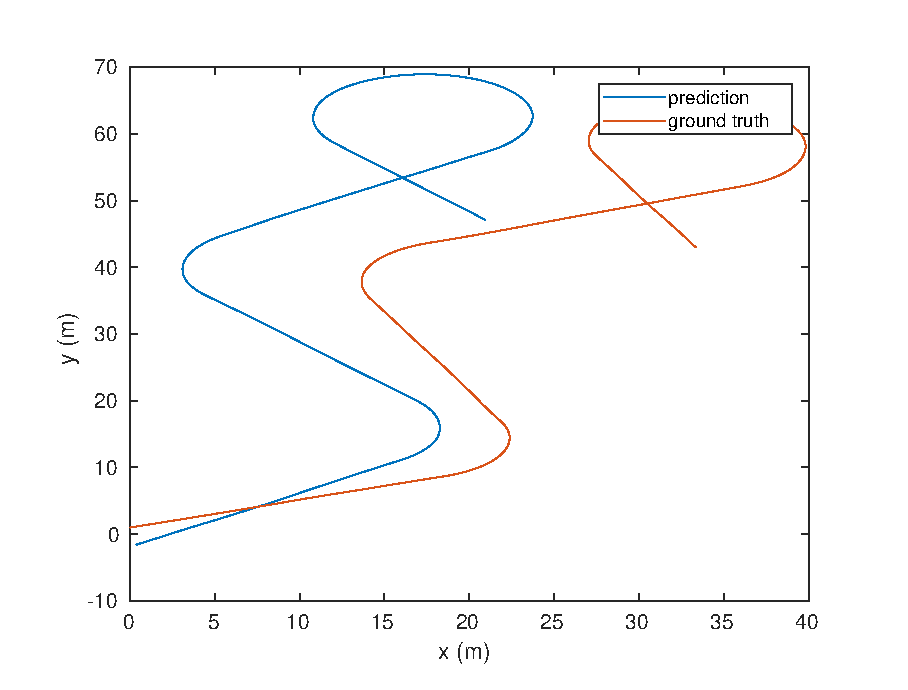
\includegraphics[width=\maxwidth{83.69292523833417em}]{figure_0.eps}
\end{center}


\vspace{1em}
\matlabheadingtwo{1. c. ii. Fully Extended Kalman Filter}

\begin{matlabcode}
clear q_hat
% define placeholder for states and P
q_hat = zeros(3,2501);


% define the intitial state estimate
q_hat(:,1) = [0.355 ; -1.590; 0.682];

H = [1 0 0; 0 1 0];

% iterate over 2500 time entries (defined as time_duration)
for t1 = 1:time_duration-1
    % prediction step
    v = mvnrnd([0;0], V);

    q_hat(:,t1+1) = [ q_hat(1,t1) + timestep.*(u(1,t1) + v(1)).*cos(q_hat(3,t1)); 
                   q_hat(2,t1) + timestep.*(u(1,t1) + v(1)).*sin(q_hat(3,t1));
                   q_hat(3,t1) + timestep.*((u(2,t1) + v(2)))]; % eq. 8.37
    if mod(t1,10) == 0
        % time is not absolute time, but just an index position
        time = t1/10;
        
        % calculate the F matrix:
        F = [1 0 -timestep*u(1,t1)*sin(q_groundtruth(3,t1));
             0 1 timestep*u(1,t1)*cos(q_groundtruth(3,t1));
             0 0 1];

        gamma = [timestep*cos(q_groundtruth(3,t1))  0;
                 timestep*sin(q_groundtruth(3,t1))   0;
                 0                          timestep];
        
        P = F*P*transpose(F) + gamma*V*transpose(gamma); % eq. 8.38
        S = H*P*transpose(H) + W; % eq. 8.43
        R = P*(transpose(H))*inv(S); % eq. 8.44

        % RECHECK THIS!!! (should be actual - predicted value)
        v2 = y(:,time) - q_hat(1:2,t1+1); % eq. 8.42

        P = P - R*H*P;
        q_hat(:,t1+1) =  q_hat(:,t1+1) + R*v2;
    end
end
% EKF estimates
plot(q_hat(1,:), q_hat(2,:))
hold on
% ground truths
plot(q_groundtruth(1,:), q_groundtruth(2,:))
% GPS measurements
scatter(y(1,:), y(2,:))
hold off
ylabel('y (m)')
xlabel('x (m)')
legend({'prediction', 'ground truth', 'GPS measurement'})
\end{matlabcode}
\begin{center}
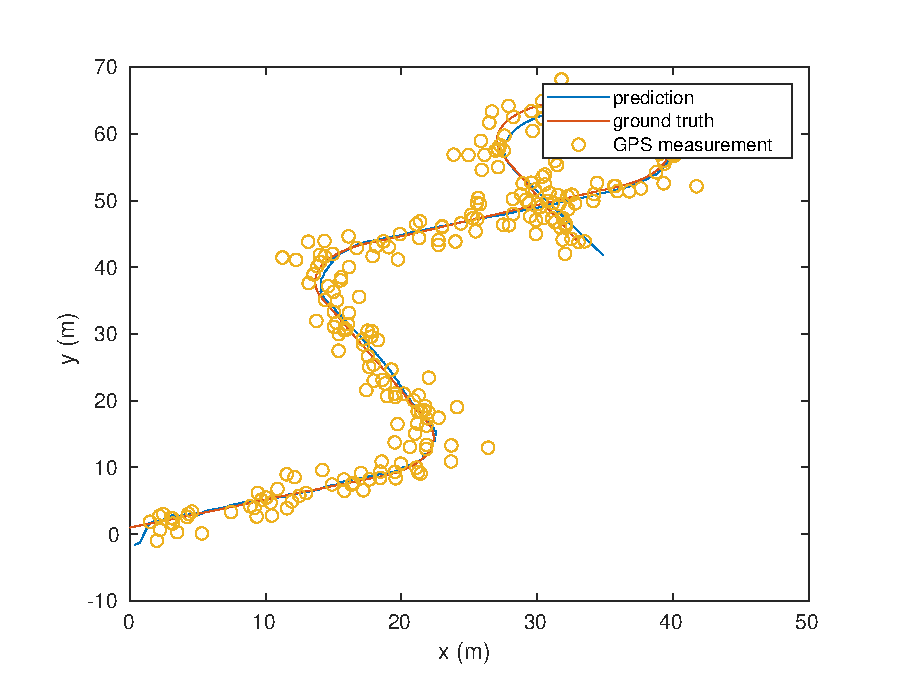
\includegraphics[width=\maxwidth{83.69292523833417em}]{figure_1.eps}
\end{center}


\vspace{1em}
\begin{par}
\begin{flushleft}
Scaling W down by a factor of 100
\end{flushleft}
\end{par}

\begin{matlabcode}
clear W
W = [1.8817 0.0632; 0.0632 2.1384]*0.01
\end{matlabcode}
\begin{matlaboutput}
W = 2x2    
    0.0188    0.0006
    0.0006    0.0214

\end{matlaboutput}
\begin{matlabcode}

clear q_hat
% define placeholder for states and P
q_hat = zeros(3,2501);


% define the intitial state estimate
q_hat(:,1) = [0.355 ; -1.590; 0.682];

H = [1 0 0; 0 1 0];

% iterate over 2500 time entries (defined as time_duration)
for t1 = 1:time_duration-1
    % prediction step
    v = mvnrnd([0;0], V);

    q_hat(:,t1+1) = [ q_hat(1,t1) + timestep.*(u(1,t1) + v(1)).*cos(q_hat(3,t1)); 
                   q_hat(2,t1) + timestep.*(u(1,t1) + v(1)).*sin(q_hat(3,t1));
                   q_hat(3,t1) + timestep.*((u(2,t1) + v(2)))]; % eq. 8.37
    if mod(t1,10) == 0
        % time is not absolute time, but just an index position
        time = t1/10;
        
        % calculate the F matrix:
        F = [1 0 -timestep*u(1,t1)*sin(q_groundtruth(3,t1));
             0 1 timestep*u(1,t1)*cos(q_groundtruth(3,t1));
             0 0 1];

        gamma = [timestep*cos(q_groundtruth(3,t1))  0;
                 timestep*sin(q_groundtruth(3,t1))   0;
                 0                          timestep];
        
        P = F*P*transpose(F) + gamma*V*transpose(gamma); % eq. 8.38
        S = H*P*transpose(H) + W; % eq. 8.43
        R = P*(transpose(H))*inv(S); % eq. 8.44

        % RECHECK THIS!!! (should be actual - predicted value)
        v2 = y(:,time) - q_hat(1:2,t1+1); % eq. 8.42

        P = P - R*H*P;
        q_hat(:,t1+1) =  q_hat(:,t1+1) + R*v2;
    end
end
% EKF estimates
plot(q_hat(1,:), q_hat(2,:))
hold on
% ground truths
plot(q_groundtruth(1,:), q_groundtruth(2,:))
% GPS measurements
scatter(y(1,:), y(2,:))
hold off
ylabel('y (m)')
xlabel('x (m)')
legend({'prediction', 'ground truth', 'GPS measurement'})
\end{matlabcode}
\begin{center}
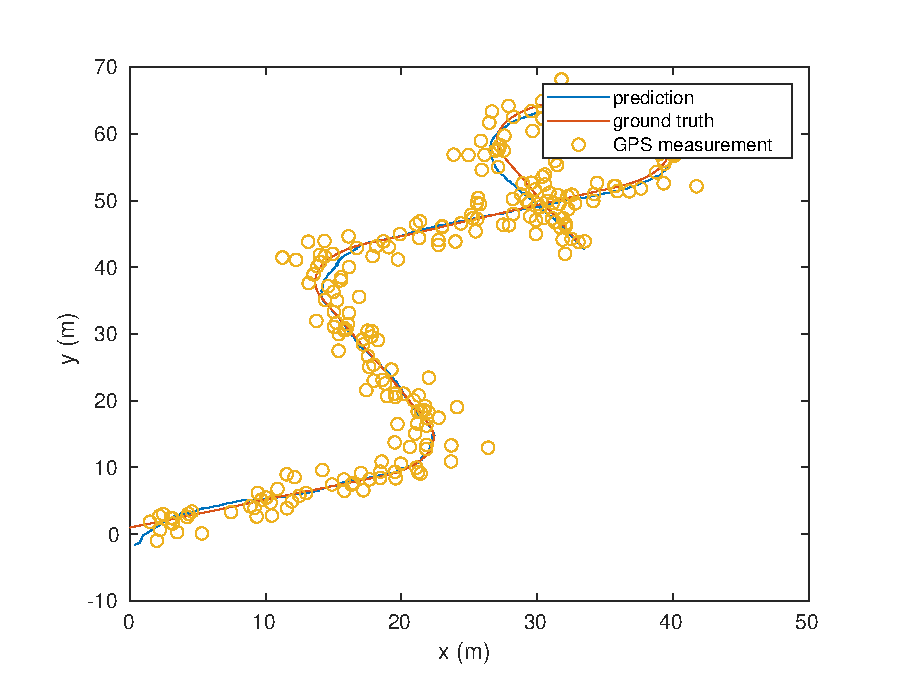
\includegraphics[width=\maxwidth{83.69292523833417em}]{figure_2.eps}
\end{center}

\end{document}
